\chapter{The Norwegian Young Sea Ice Field Campaign}
\vspace{1 cm}
\begin{spacing}{1} \begin{quote} 
\noindent \emph{Earth system observations are an essential driver of progress in our understanding of climate change. Overall, capabilities to observe the physical climate system have continued to improve and expand. Improvements are particularly evident in ocean observing networks and remote-sensing systems.} \end{quote}
\hspace{6 cm} - IPCC Sixth Assessment Report, August 2021  
\end{spacing}
\doublespacing
\section{Introduction}
The Norwegian Young Sea Ice field campaign (N-ICE2015 or N-ICE) was a 6-month field campaign conducted from January to July 2015, observing both atmospheric properties and sea ice dynamics. During this period, a Norwegian research vessel, the RV Lance, was frozen into the sea ice north of Svalbard and allowed to move with the ice floes. The ship tracks can be seen in Figure \ref{fig:nice}. Three times during the expedition the ice surrounding the ship broke up and the ship needed to be repositioned into the sea ice. The time it took for the ship to reposition can be seen as gaps in the data from 21 February, through 24 February, 15 March through 24 April, and again from 5 June through 7 June. The period in March and April corresponds with a trip back to Svalbard for resupply, explaining the long duration of the data gap. The dates of each ice floe are listed in Table \ref{tab:floedates}. 

\begin{figure}[b!]
    \centering
    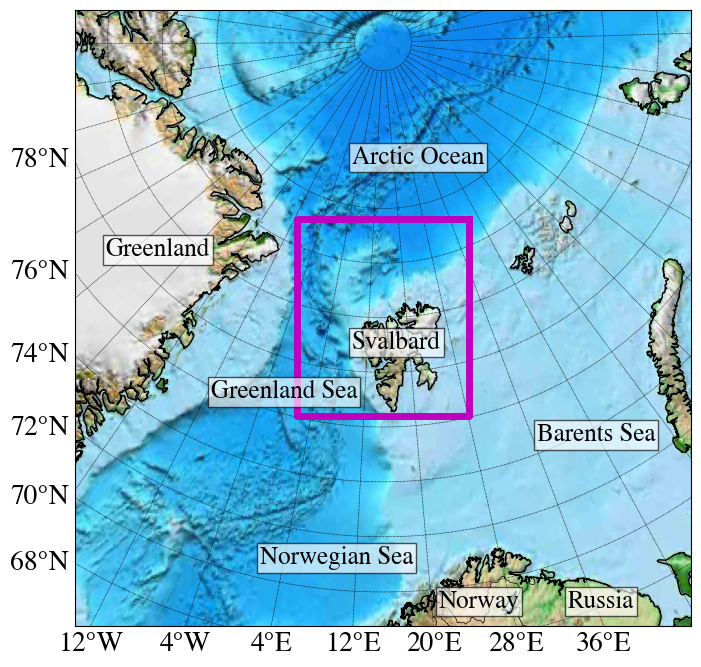
\includegraphics[width=0.5\linewidth]{figures/chapter2/ship_zoom_out.png}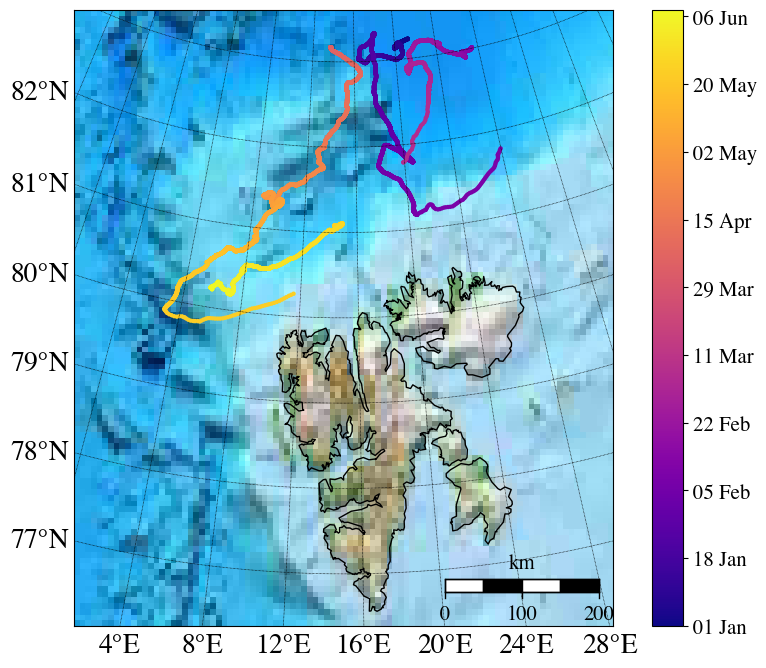
\includegraphics[width=0.55\linewidth]{figures/chapter2/ship_zoom_in.png}
    \caption[N-ICE location.]{The location of the N-ICE field expedition. The right map shows a detailed view of the area indicated by the purple box on the left map. Ship location is plotted on the right figure and is colored by date.}
    \label{fig:nice}
\end{figure}

\begin{table}[t!]
\centering
\footnotesize
\doublespacing
{
\begin{tabular}{| c | c | c | c | c  |}
 \hline
\rowcolor[HTML]{F3F3F3}  &  &  & \multicolumn{2}{ c |}{\textbf{Ice Edge Proximity}} \\
\rowcolor[HTML]{F3F3F3} 
\multirow{-2}{*}{\textbf{Floe}} & \multirow{-2}{*}{\textbf{Start Date}} & \multirow{-2}{*}{\textbf{End Date}} & \textbf{Min Distance} & \textbf{Max Distance} \\
  \hline
 1 & 15 January 2015 & 21 February 2015 & 50 km & 175 km\\
 2 & 24 February 2015 & 19 March 2015 & 200 km & 325 km\\ 
 3 & 18 April 2015 & 5 June 2015 & 225 km & 40 km \\
 4 & 7 June 2015 & 21 June 2015 & 85 km & 10 km \\
  \hline
\end{tabular}}
\caption[N-ICE floe dates and ice edge proximity.]{Floe dates and approximate proximity to ice edge for the N-ICE field campaign.}
\label{tab:floedates}
\end{table}

This region is characterized by thin, first-year (or ``young") sea ice, as opposed to the thick, multi-year sea ice observed during SHEBA \citep{cohen:2017}. As a result, the N-ICE measurements are representative of the new regime that the polar regions are moving toward as the climate warms. This expedition is of particular interest from a modeling perspective due to the magnitude of the temperature and pressure change during and after winter storm periods. This research cruise is the first to take seasonal measurements of the clouds and atmosphere since SHEBA in 1997 and 1998. These concurrent measurements of the energy budget and cloud properties (fraction, height, microphysical, and temperature) can give important insight into climate processes and radiative transfer \citep{persson:2002, schweiger:2004}. 

\citet{shupe:2004} observed mixed-phase clouds during SHEBA were consistent in temperature, liquid water path, and ice water content with previous studies over similar sea ice. NICE2015 observed more extreme storm periods than those seen at SHEBA, bringing wind speed, pressure, and temperature changes of previously unobserved magnitudes. In general, the winter during N-ICE was characterized by several significant storm periods \citep{cohen:2017}. These storms were associated with significant changes in surface temperature and humidity conditions, as well as changes in cloud properties. Springtime conditions during N-ICE were less stormy, with a gradual increase in surface temperatures and fairly constant thick cloud cover \citep{cohen:2017}.

Throughout much of N-ICE, strong temperature inversions were observed over the surface, similar to what was seen at SHEBA \citep{kayser:2017}. While these strong inversions are not unique to N-ICE2015, they are often underrepresented in Polar WRF simulations \citep{hines:2015}. 
\newline 
\noindent The primary objectives of N-ICE are:
\begin{enumerate}
    \item To quantify the change in atmosphere-ice-ocean interactions as the atmosphere shifts from primarily multi-year sea ice to thin, first-year sea ice \citep{granskog:2018, granskog:2015}. 
    \item To observe how changes in sea ice impact the marine ecosystem and their response \citep{granskog:2015}.
    \item To provide key observations to tune and validate models \citep{granskog:2018, granskog:2015}.
\end{enumerate}

 The overall conditions during the field campaign are described by \citet{cohen:2017}, \citet{kayser:2017}, and \citet{walden:2017}. More details about the experiment and the datasets that were collected can be found in \citet{granskog:2015}. \citet{itkin:2017} describes the proximity to the sea ice edge throughout the experiment. During the majority of the experiment, the ship was stationed between 50 and 250 $km$ from the ice edge during the first 3 floes. Approximate distances to the ice edge during each floe are listed in Table \ref{tab:floedates} \citep{oikkonen:2017}.

\section{Instruments}
A variety of instruments were deployed during the N-ICE campaign and provided data that will be used in this project, including radiosondes, a MicroPulse Lidar (MPL), a meteorological tower, an eddy covariance (EC) system, and broadband shortwave and longwave radiometers. 

Vaisala RS92-SGP radiosondes were launched from the ice surface (Floe 1) or the ship deck (Floes 2, 3, and 4) twice daily around 1100 and 2300 UTC. The radiosondes recorded temperature, relative humidity, wind speed and direction, pressure, and geopotential height as high as 30 $km$. Data were recorded by the radiosondes every two seconds and were transmitted to the ground using a Vaisala MW31 ground station \citep{kayser:2017, cohen:2017}. More information and analysis of the radiosondes can be found in \citet{kayser:2017}.

Data from the MPL were recorded every 14 seconds up to a height of 18 $km$. The MPL records backscattered light from clouds and operates at 532 $nm$. The range resolution is 15 m, with an 18 km maximum cloud base height. Distance uncertainties are $\pm$ 2$\%$ due to timing uncertainties within the instrument. This instrument is more sensitive to water particles than ice, so some cloud types may be biased toward higher percentages of water than ice within the cloud. The MPL is easily attenuated by optically thick clouds. In some instances when a low water cloud is detected, it is possible that more cloud layers exist above this layer that cannot be measured by the MPL. 

A meteorological tower was deployed on the ice 300 to 400 $m$ away from the ship. This tower was set up within a few days of anchoring to each new floe and recorded relative humidity and temperature (Vaisala HMP155), and wind speed and direction (Lufft Ventus V200A-UMB) at 2, 4, and 10 $m$ heights. Pressure (RM Young 61302 V) was measured at 1.5 $m$. All measurements were collected by a Campbell Scientific CR30000 data logger at 1-second resolution. Periods of missing tower data were reconstructed using temperature and wind information from the ship (sensors mounted 22 to 24 $m$ above the surface). More information about the meteorological measurements, temperature, and wind reconstruction using the ship data, a diagram of the meteorological tower setup, and a comparison of the meteorology to SHEBA can be found in \citet{cohen:2017}.

Radiometers (Kipp and Zonen CMP22 and CGR4) were set up 1 to 1.2 $m$ above the surface near the meteorological tower to measure upward and downward components of longwave and shortwave radiation. Kipp and Zonen CVF4 ventilation units were used to heat and ventilate the radiometers to avoid riming and frosting of the radiometer domes. More information about the radiometers and an analysis of the surface energy budget can be found in \citet{walden:2017}.

Turbulent flux data were collected by a closed path EC flux system (Campbell CPEC200) mostly at  20 $Hz$ (but occasionally 10 $Hz$). This system contains a sonic anemometer and a closed-path, infrared gas analyzer. These instruments allow observation of the heat and moment exchanges and the water vapor and carbon dioxide mixing ratios, respectively. This system was set up next to the meteorological tower over a snow-covered surface. Further information about the EC Flux system can be found in \citet{walden:2017}.

\section{Atmospheric components of the surface energy budget over young sea ice}
\citet{walden:2017} detailed the turbulent and radiative fluxes over thin sea ice during N-ICE. Snow albedo was around 0.85 in the winter and between 0.72 and 0.80 in the spring and summer. Stable stability was found in the winter, followed by unstable conditions in the spring, and approximately neutral stability in the summer (once the skin temperature reached 0$^{\circ}C$). Latent and sensible heat flux values ranged between -10 to +10 $Wm^{-2}$ and -100 to +100 $Wm^{-2}$, respectively, in both the winter and spring. Shortwave radiation was not seen at the field site until March, at which time the sun rose and shortwave radiation increased until downward values reached almost 800 $Wm^{-2}$ mid-day near the end of the experiment. Downward longwave radiation ranged from 110 to 125 $Wm^{-2}$ during clear-sky times, and reached around 300 $Wm^{-2}$ under cloudy conditions. Positive values of net radiation and turbulent fluxes indicate flux into the surface.

Murphy's contribution to \cite{walden:2017} was to solve several problems with the flux dataset collected during the N-ICE campaign and to process the data through the EddyPro software. The most restrictive data problem was the number of data gaps throughout 30-minute data files, which was caused by a programming error in the datalogger. In some cases, the amount of missing data made the file unable to be processed. To fix this, the data were filled by taking the section of data before it (or after, in the case that the missing data was too close to the start of the dataset) and replicating it for the time period with no recorded data. To ensure that this method of data filling was acceptable, data from the Barrow, Alaska DOE ARM site (https://www.arm.gov/capabilities/observatories/nsa) was used to compare the post-processed data of a complete dataset with the post-processed results from the same dataset after (artificially added) gaps had been filled. Analysis of both the difference in sensible heat fluxes and the turbulent spectra from before and after the data filling were examined and determined the filling method appropriate for the type of gaps in the N-ICE data. Details of this gap-filling study were written as a report for a course on flux measurements. This report can be seen in Appendix B. 